\section{Processi primari}
\subsection{Fornitura}
    \subsubsection{Scopo}
        Il processo di fornitura sostanzialmente si occupa della gestione dei rapporti con il cliente.
        Il suo scopo quindi è quello di determinare strumenti e competenze utili e necessari alla realizzazione del prodotto e di assicurare la conformità di questo con le richieste del proponente. Si rende necessaria quindi la produzione di documenti che descrivano le intenzioni e le modalità che il gruppo si prefigge di seguire al fine di soddisfare il cliente.
    \subsubsection{Aspettative}
        Il confronto diretto e frequente tra fornitore e proponente è senza dubbio utile ad entrambe le parti, affinché ambedue soddisfino i loro obiettivi in tempi desiderabili.
    \subsubsection{Descrizione}
        Il processo di fornitura si compone \hfoot{Standard ISO 12207 \S\ 5.2} di 7 attività\textsubscript{G}, definite come segue:
    \subsubsection{Attività}
        \pparagraph{Inizializzazione}
            Il gruppo dovrà effettuare collettivamente una valutazione di tutti i capitolati\textsubscript{G} proposti e formalizzarla in uno \textsc{studio di fattibilità}, il quale, per ogni capitolato\textsubscript{G}, darà una breve descrizione dello stesso, delle finalità, delle tecnologie, degli aspetti positivi e delle criticità, proponendo poi delle conclusioni che saranno il frutto delle riflessioni interne ed indicando la scelta definitiva dei membri.

        \pparagraph{Preparazione della risposta}
            Il gruppo preparerà una lettera di presentazione indirizzata al committente ed al proponente del capitolato\textsubscript{G} scelto, per candidarsi alla fornitura del prodotto indicando un sunto del preventivo dei costi.

        \pparagraph{Pianificazione}
        \label{pianificazione}
            Il gruppo dovrà fornire dei documenti che illustrino la gestione del lavoro e mostrino come verranno assicurati qualità e conformità del prodotto. Nello specifico realizzerà:
            \begin{itemize}
                \item un \textsc{piano di progetto}, contenente \footnote{\url{https://www.math.unipd.it/~tullio/IS-1/2020/Dispense/FC2.pdf} \S\ 3}:
                    \begin{itemize}
                        \item \textbf{pianificazione macroscopica (a lungo periodo):}
                        \begin{itemize}
                            \item scadenze, fissate all'indietro;
                            \item analisi dei rischi;
                            \item preventivo dei costi.
                        \end{itemize}

                        \item \textbf{pianificazione dettagliata (a breve):}
                        \begin{itemize}
                            \item attività\textsubscript{G}, fissate in avanti;
                            \item preventivo minuto, alla luce del consuntivo di periodo\textsubscript{G} precedente;
                            \item riscontro dei rischi ed aggiornamento delle misure di mitigazione.
                        \end{itemize}

                    \end{itemize}

                    che andrà così strutturato: \footnote{\url{https://www.math.unipd.it/~tullio/IS-1/2020/Dispense/L06.pdf} \S\ 25}:
                    \subitem -- Introduzione (scopo e struttura);
                    \subitem -- Organizzazione del progetto\textsubscript{G};
                    \subitem -- Analisi dei Rischi;
                    \subitem -- Risorse disponibili (tempo e persone);
                    \subitem -- Suddivisione del lavoro (work breakdown);
                    \subitem -- Calendario delle attività\textsubscript{G};
                    \subitem -- Meccanismi di controllo e di rendicontazione.

                \item un \textsc{piano di qualifica}, contenente \footnote{\url{https://www.math.unipd.it/~tullio/IS-1/2020/Dispense/FC2.pdf} \S\ 4}:
                    \subitem -- obiettivi quantitativi di qualità;
                    \subitem -- cruscotto\textsubscript{G} di misurazione;
                    \subitem -- analisi degli scostamenti e misure correttive.
            \end{itemize}

        \pparagraph{Esecuzione e controllo}
            In questa attività\textsubscript{G} il gruppo \group{} dovrà implementare ed eseguire i piani delineati al punto \ref{pianificazione} e sviluppare il prodotto in accordo con il \hyperref[sviluppo]{processo di sviluppo}.

        \pparagraph{Revisione e valutazione}
            Il gruppo dovrà coordinare le revisione\textsubscript{G} delle attività\textsubscript{G} svolte e gestire la comunicazione con il committente ed il proponente. Si dovrà inoltre aver cura di operare in accordo con quanto scritto negli altri processi.


        \pparagraph{Consegna e completamento}
            Il fornitore dovrà consegnare il prodotto in accordo con quanto specificato nel contratto. A seguito della consegna del prodotto, il gruppo \group{}  non si farà carico delle mansioni di supporto ed assistenza.

\clearpage
\subsection{Sviluppo}
\label{sviluppo}
    \subsubsection{Scopo}
        Il processo di sviluppo comprende tutte quelle attività\textsubscript{G} che portano alla costruzione del prodotto finale.
    \subsubsection{Aspettative}
        Questo processo dev'essere attuato secondo quanto pattuito con proponente e committente, rispettando i loro requisiti\textsubscript{G} e soddisfacendo le loro aspettative. Tutto ciò naturalmente rispettando le norme definite in questo documento.
    \subsubsection{Descrizione}
        Nel processo di sviluppo si individuano \hfootiso{5.3} le seguenti attività\textsubscript{G}:

    \subsubsection{Attività}
        \paragraph{Analisi dei requisiti}
            \ssubparagraph{Descrizione}
                Gli analisti devono stabilire, raccogliere e documentare tutti i requisiti\textsubscript{G} stilando un documento che fornirà una base precisa su cui i progettisti si potranno fondare. Dovrà contenere, in accordo con quanto richiesto dal cliente, la raccolta dei casi d'uso\textsubscript{G}, rappresentati anche tramite diagrammi UML\textsubscript{A}, ed il tracciamento di tutti i requisiti\textsubscript{G} individuati.

            \ssubparagraph{Nomenclatura casi d'uso}
                Ogni caso d'uso\textsubscript{G} è univocamente identificato da un codice, secondo lo schema:
                $$\text{UC[caso].[sottoCaso].[sottoSottoCaso].[sottoSottoSottoCaso]}$$
                dove caso ed i successivi sono numeri progressivi che partono da 1, solo il primo è obbligatorio. Segue poi un breve nome. Inoltre ogni caso dovrà avere le seguenti sezioni (quelle indicate tra parentesi (...) sono opzionali):
                \begin{itemize}
                    \item attori\textsubscript{G} primari;
                    \item (attori secondari);
                    \item descrizione;
                    \item (estensioni);
                    \item (inclusioni);
                    \item precondizione\textsubscript{G};
                    \item post condizione\textsubscript{G};
                    \item scenario\textsubscript{G} principale, uno solo per caso d'uso\textsubscript{G}, rappresenta il normale flusso degli eventi;
                    \item (scenari alternativi).
                \end{itemize}

                Tutti i casi d'uso\textsubscript{G} non banali verranno accompagnati da diagrammi secondo lo standard UML\textsubscript{A} 2.0 \footnote{\url{https://www.omg.org/spec/UML/2.0/Superstructure/PDF} \S\ 16} \footnote{\url{https://www.math.unipd.it/~rcardin/swea/2021/Diagrammi\%20Use\%20Case_4x4.pdf}}.
                Questo è un esempio di caso d'uso\textsubscript{G} conforme alle regole appena definite:
                \begin{figure}[H]
                    \centering
                    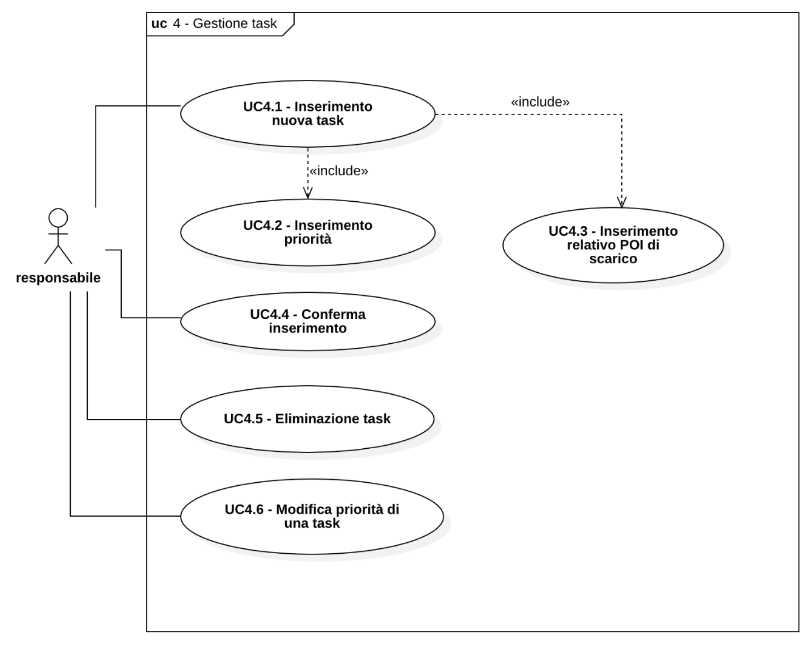
\includegraphics[scale=0.5]{res/images/esempio_use_case.png}
                    \caption{Esempio di caso d'uso}
                \end{figure}

            \ssubparagraph{Classificazione dei requisiti}
                Per favorire l'organizzazione ed il tracciamento dei requisiti\textsubscript{G}, questi saranno classificati secondo la convenzione che segue:
                $$\text{R[tipo]-[numero progressivo]-[importanza]}$$
                dove tipo è uno tra:
                \begin{itemize}
                    \item \textbf{V}$\rightarrow$ vincolo;
                    \item \textbf{F}$\rightarrow$ funzionale;
                    \item \textbf{Q}$\rightarrow$ qualità;
                    \item \textbf{P}$\rightarrow$ prestazionale;
                \end{itemize}
                mentre importanza può essere:
                \begin{itemize}
                    \item \textbf{O}$\rightarrow$ obbligatorio, irrinunciabile per qualcuno degli stakeholder\textsubscript{G};
                    \item \textbf{D}$\rightarrow$ desiderabile, non strettamente necessario, ma se ne riconosce il valore aggiunto;
                    \item \textbf{F}$\rightarrow$ facoltativo, relativamente utile oppure contrattabile in futuro.
                \end{itemize}
                Il numero progressivo parte da 1 ed i sotto requisiti\textsubscript{G} si indicano in maniera analogo ai sotto casi d'uso\textsubscript{G}.

        \paragraph{Progettazione}
            \ssubparagraph{Descrizione}
                I progettisti hanno il compito di tradurre il problema in una possibile soluzione, descritta come architettura, da dividere in parti che possono essere trattate individualmente. Sarà necessario:
                \begin{itemize}
                    \item svolgere le attività\textsubscript{G} coerentemente con quanto individuato nell'analisi dei requisiti\textsubscript{G};
                    \item adottare design pattern\textsubscript{G} opportuni quando si individuano strutture che ne possono trarre beneficio;
                    \item seguire i principi SOLID\footnote{\url{https://www.math.unipd.it/~rcardin/swea/2021/SOLID\%20Principles\%20of\%20Object-Oriented\%20Design_4x4.pdf}};
                    \item utilizzare sempre una nomenclatura significativa, parlante e consistente.
                \end{itemize}
            \ssubparagraph{Obiettivi di qualità}
                Affinché un'architettura si possa definire buona, deve perseguire i seguenti obiettivi di qualità: \footnote{\url{https://www.math.unipd.it/~tullio/IS-1/2020/Dispense/L09.pdf} \S\ 17..27}
                \begin{itemize}
                    \item \textbf{sufficienza: }soddisfa tutti i requisiti\textsubscript{G};
                    \item \textbf{comprensibilità: }per tutti gli stakeholder\textsubscript{G};
                    \item \textbf{modularità: }suddivisa in parti chiare e ben distinte;
                    \item \textbf{robustezza: }capace di sopportare ingressi diversi da utenti ed ambienti differenti;
                    \item \textbf{flessibilità: }permette modifiche a costo contenuto al variare dei requisiti\textsubscript{G};
                    \item \textbf{riusabilità: }le sue parti possono essere impiegate in altre applicazioni;
                    \item \textbf{efficienza: }nel tempo (CPU), nello spazio (RAM), nelle comunicazioni (rete);
                    \item \textbf{affidabilità: }svolge bene il suo compito quando utilizzata con un'alta probabilità;
                    \item \textbf{disponibilità: }la sua manutenzione la rende indisponibile per un tempo ridotto;
                    \item \textbf{safety\textsubscript{G} };
                    \item \textbf{security\textsubscript{G} };
                    \item \textbf{semplicità: }ogni parte contiene solo il necessario e niente di superfluo;
                    \item \textbf{incapsulazione: }l'interno delle componenti non è visibile all'esterno;
                    \item \textbf{coesione: }le parti che stanno insieme hanno gli stessi obiettivi;
                    \item \textbf{basso accoppiamento: }parti distinte hanno una dipendenza il più possibile ridotta.
                \end{itemize}
            \ssubparagraph{Attività}
                La progettazione porterà in seguito alla produzione di una Technology Baseline\textsubscript{G} e di una Product Baseline\textsubscript{G}. A supporto di queste, ci saranno diversi diagrammi, sempre secondo lo standard UML\textsubscript{A} 2.0:
                \begin{itemize}
                    \item \textbf{delle classi\footnote{\url{https://www.math.unipd.it/~rcardin/swea/2021/Diagrammi\%20delle\%20Classi_4x4.pdf}}: }per rappresentare oggetti e relazioni tra questi in un sistema;
                    \item \textbf{dei package\footnote{\url{https://www.math.unipd.it/~rcardin/swea/2021/Diagrammi\%20dei\%20Package_4x4.pdf}}: }per rappresentare dipendenze tra classi e package ad un livello di astrazione più alto rispetto a quello dei diagrammi delle classi;
                        \item \textbf{delle attività\footnote{\url{https://www.math.unipd.it/~rcardin/swea/2021/Diagrammi\%20di\%20Attivit\%c3\%a0_4x4.pdf}}: }per descrivere processi o algoritmi;
                    \item \textbf{di sequenza\footnote{\url{https://www.math.unipd.it/~rcardin/swea/2021/Diagrammi\%20di\%20Sequenza_4x4.pdf}}: }la collaborazione di un gruppo di oggetti che devono implementare collettivamente un comportamento.
                \end{itemize}
                Si dovranno indicare le tecnologie che si andranno ad utilizzare, descrivendo il loro impiego e le motivazioni che hanno portato alla loro scelta.
        \pparagraph{Codifica}
            Qui si definiscono le norme che i programmatori dovranno seguire, di modo da:
             \begin{itemize}
                 \item perseguire: leggibilità, uniformità e consistenza;
                 \item agevolare: verifica, validazione e manutenzione.
             \end{itemize}
             \ssubparagraph{Convenzioni}
             Per uniformare lo stile di codifica all'interno del gruppo si seguono le linee guida di Google per i vari linguaggi adottati:
             \begin{itemize}
                 \item java: \\\url{https://google.github.io/styleguide/javaguide.html};
                 \item javascript: \\\url{https://google.github.io/styleguide/jsguide.html};
                 \item typescript: \\\url{https://google.github.io/styleguide/tsguide.html};
                 \item JSON: \\\url{https://google.github.io/styleguide/jsoncstyleguide.xml};
                 \item HTML/CSS: \\\url{https://google.github.io/styleguide/htmlcssguide.html}.
             \end{itemize}

            \ssubparagraph{Strumenti}
            Viene adottato l'editor di testo Visual Studio Code \footnote{Documentazione VS Code: \url{https://code.visualstudio.com/docs}} in quanto molto leggero ma allo stesso tempo ricco e potente grazie all'ampio ventaglio di estensioni e plugin a disposizione. Inoltre è ugualmente disponibile per Linux, MacOS e Windows.\\
            Per il rispetto delle regole sopracitate e per automatizzare la formattazione uniforme del codice si adottano gli strumenti:
            \begin{itemize}
                \item spotless per java, configurabile come plugin gradle:
                    \subitem -- \url{https://github.com/diffplug/spotless/tree/master/plugin-gradle};
                \item prettier per tutti gli altri linguaggi, installabile ed utilizzabile tramite npm\textsubscript{A}:
                    \subitem -- \url{https://prettier.io/docs/en/index.html}.
            \end{itemize}








    %\subsubsection{Strumenti}









